% Full conference draft with results from archived experiments.
% ISCAS 2026 specifies IEEEtran in conference mode.
\documentclass[conference,letterpaper]{IEEEtran}
\usepackage{amsmath,amssymb}
\usepackage{cite}
\usepackage{graphicx,booktabs}
\usepackage{flushend}
\usepackage[hidelinks]{hyperref}
\title{DiMA-PPI: Canonical State-Potential Learning\\
for Consistent Protein Binding Mutation Prediction}
% Names and institutional mapping are inherited from the existing manuscript.
% Author approval and the final affiliation wording remain the authors' responsibility.
\author{\IEEEauthorblockN{Qi Liu\IEEEauthorrefmark{1},
Xinyi Xu\IEEEauthorrefmark{1}, Qian Cheng\IEEEauthorrefmark{1},
Chen Wu\IEEEauthorrefmark{1}, Lu Meng\IEEEauthorrefmark{1},
Defu Yang\IEEEauthorrefmark{2}, Xinbo Gao\IEEEauthorrefmark{1},
and Xueli Chen\IEEEauthorrefmark{1}\IEEEauthorrefmark{2}}
\IEEEauthorblockA{\IEEEauthorrefmark{1}Xidian University, Xi'an, China\\
\IEEEauthorrefmark{2}Hangzhou Normal University, Hangzhou, China\\
Correspondence: xyxu@xidian.edu.cn; xbgao@mail.xidian.edu.cn; xlchen@xidian.edu.cn}}
\begin{document}
\maketitle
\begin{abstract}
Predicting mutation-induced changes in protein--protein binding free energy
supports variant interpretation and protein engineering. Independently
predicted substitution effects can produce path-dependent estimates of the
binding free-energy difference between the same protein variants. We propose
DiMA-PPI, a multimodal graph neural network that enforces path consistency
through shared state-potential learning. The model integrates sequence
embeddings, structural representations and local atomic descriptors to
estimate latent potentials for bound and isolated-chain states. Mutation
effects are expressed as differences between the binding potentials of the
initial and final variants. Canonical state reuse maintains a single
numerical value for each represented state across all predictions.
On S1129, comprising 1,129 substitutions from 111 complexes,
DiMA-PPI achieves a Pearson correlation coefficient (PCC) of 0.757 and a root mean
squared error (RMSE) of 1.542~kcal mol$^{-1}$. We further construct PPI-Path92,
which contains 92 groups of same-site variants and 9,904 mutant-to-mutant
comparisons whose targets are derived from measured effects relative to the
wild type.
On PPI-Path92, DiMA-PPI achieves an RMSE of 1.611~kcal mol$^{-1}$ and a mean
discrepancy of $4.78\times10^{-7}$~kcal mol$^{-1}$ between direct and
multistep predictions. Experiments with fixed model parameters show that
state reuse eliminates inconsistencies arising from independent stochastic
evaluation and reduces redundant computation. These results support
canonical state-potential learning for consistent prediction of binding
changes across related protein variants.
\end{abstract}
\begin{IEEEkeywords}
Graph neural networks, state potentials, protein binding, path consistency.
\end{IEEEkeywords}

\section{Introduction}
Predicting changes in protein--protein binding free energy following
amino-acid substitution is a central task in variant interpretation and
protein engineering. Established tools include FoldX~\cite{foldx},
MutaBind2~\cite{mutabind2}, mCSM-PPI2~\cite{mcsmppi2} and
DDMut-PPI~\cite{ddmutppi}. Graph neural networks and pretrained protein
representations integrate structural and sequence information to estimate
these effects~\cite{graphppi,dssappi}. Evaluation on benchmarks such as
SKEMPI~\cite{skempi2} primarily measures accuracy for individual substitutions.
Comparison of related variants additionally requires path consistency:
for states $a$, $b$ and $c$ under the same modeled conditions, the predicted
change from $a$ to $c$ should equal the sum of the changes from $a$ to $b$
and from $b$ to $c$. This relation couples predictions across substitutions.

Reverse-mutation augmentation and antisymmetric prediction address
directional bias~\cite{ddgbias} by relating each substitution to its reverse.
Global consistency additionally requires zero accumulated change around
closed mutation cycles. Representing protein states as graph nodes and
mutation effects as directed edges provides a unified formulation: edge
values defined by node-potential differences sum to zero around every cycle,
analogous to voltage differences around a circuit loop. Implementing this
property requires identical numerical representations of shared states
throughout structure preparation and inference.

StaB-ddG derives binding effects from folding scores~\cite{stabddg}, while
DSSA-PPI uses residue-score differences under a shared conditioning
context~\cite{dssappi}. We introduce canonical state identity across
structure preparation, feature extraction and inference to preserve
potential differences throughout the prediction pipeline.
DiMA-PPI learns a binding potential from each pair of bound and free
representations and reuses canonical state values across mutation queries.
We also construct PPI-Path92 from S1129 to evaluate compositional prediction
and cycle consistency. Matched model comparisons assess the relationship
between predictive accuracy and consistency, while experiments with fixed
model parameters quantify the numerical and computational effects of state
reuse.

\section{Proposed Method}
\label{sec:method}
\begin{figure*}[t]
 \centering
 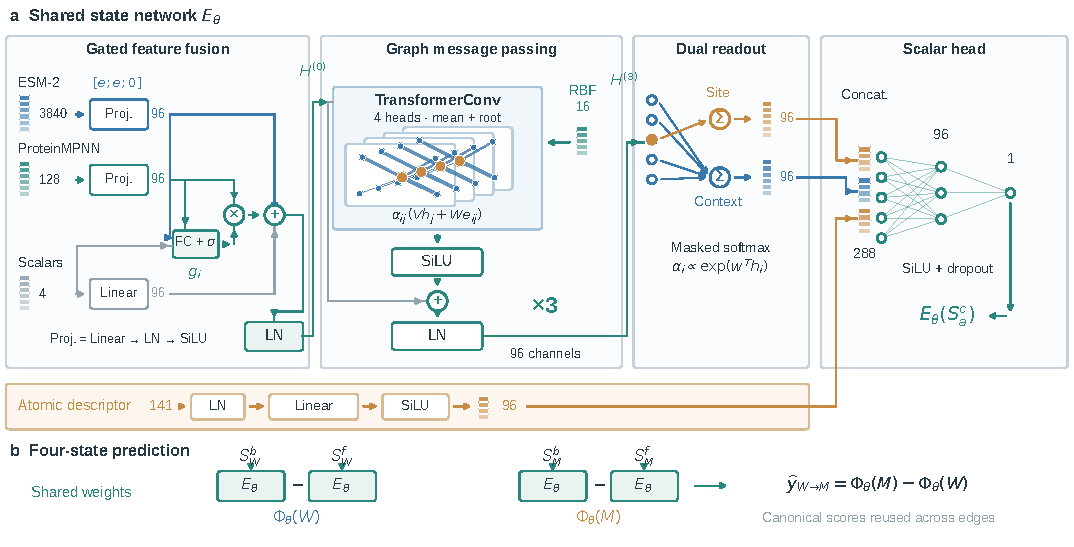
\includegraphics[width=\textwidth]{fig_model.pdf}
 \caption{DiMA-PPI network architecture. (a) Projected sequence and backbone
 features enter a learned sigmoid gate; elementwise multiplication and addition
 form the fused node features. Each of three graph blocks contains four-head
 TransformerConv, SiLU, a residual addition and LayerNorm (LN). Edge RBFs enter
 attention; line widths schematically indicate attention weights. Masked
 attention pools the mutation site and context separately. Their two 96-D
 vectors are concatenated with a projected 96-D atomic descriptor and passed
 through a 288--96--1 scalar head. Drawn neurons represent layers rather than
 exact neuron counts. (b) The same network scores all four bound/free and
 WT/mutant states. Bound-minus-free scores define binding potentials, whose
 difference gives the mutation effect. Canonical scores are reused across edges.}
 \label{fig:model}
\end{figure*}
Figure~\ref{fig:model} summarizes the shared encoder, four-state output and
canonical inference procedure.
\subsection{Canonical Bound and Free States}
For a fixed complex and substitution site, $S_a$ denotes the state with
amino-acid identity $a$. Positive $y_{a\to b}=\Delta\Delta G_{a\to b}$ follows
the benchmark convention of stronger mutant binding. Each state has a bound
context $S_a^b$ and an isolated-chain free context $S_a^f$, identified by
\begin{equation}
 k(a,c)=(\text{complex},\text{chain},\text{PDB site},a,c),
 \quad c\in\{b,f\}.
\end{equation}
Each key maps to one representation selected by source-row order,
independently of labels and fold assignments. Repeated occurrences reuse
identical sequence features, graph geometry, node masks and atomic
descriptors, ensuring a consistent representation of shared intermediate
states.

The reference-backbone graph contains residues within 20~\AA{} of the site.
Edges connect residues within 8~\AA{} and sequential neighbors on each chain;
16 radial basis functions encode their distances. The bound encoder uses the
complex graph. For the free context, cross-chain edges are removed and readout
is restricted to the mutated chain. Four 141-dimensional descriptors encode
wild-type/mutant and bound/free atomic environments. PyRosetta~\cite{pyrosetta} locally repacks
side chains within 8~\AA{} in the bound structures and repacks the isolated
mutated chain for the free contexts. Descriptors contain element-distance
histograms, substituted-residue element counts, 18 residue-level Rosetta score
terms and their local sums.

\subsection{Shared Multimodal Graph Encoder}
Each residue has an ESM-2 650M embedding $e_i^a\in\mathbb{R}^{1280}$~\cite{esm2},
a ProteinMPNN reference-backbone feature $p_i\in\mathbb{R}^{128}$~\cite{proteinmpnn},
and four scalars $s_i$ encoding chain membership, site membership and
normalized site distance. The single-state sequence block is
$u_i^a=[e_i^a;e_i^a;\mathbf{0}]$, which represents a single sequence identity
in both embedding blocks and fixes the difference block to zero.
A learned gate integrates the sequence and structural features:
\begin{align}
 q_i&=\phi_{\rm seq}(u_i^a),\quad t_i=\phi_{\rm str}(p_i),\nonumber\\
 g_i&=\sigma(W_g[q_i;t_i;s_i]+b_g),\nonumber\\
 h_i^{(0)}&=\operatorname{LN}(q_i+g_i\odot t_i+W_s s_i+b_s).
\end{align}
The projections use linear layers, layer normalization and SiLU. Three
TransformerConv layers with four averaged attention heads and hidden width
96 propagate messages over the context-specific edges:
\begin{equation}
 H^{(\ell+1)}=\operatorname{LN}\!\left[H^{(\ell)}+
 \operatorname{SiLU}\big(\operatorname{TConv}_{\ell}
 (H^{(\ell)},\mathcal E_c,R)\big)\right].
\end{equation}
Attention pooling produces separate representations of the substitution
site and surrounding context, with weights proportional to
$\exp(w^\top h_i^{(3)})$ within each node set. A shared scalar head maps these
representations and the atomic descriptor to a state score:
\begin{equation}
 E_\theta(S_a^c)=\operatorname{MLP}_\theta
 ([z_{\rm site};z_{\rm context};\phi_d(d_a^c)]),
\end{equation}
where $\phi_d$ normalizes and projects the atomic descriptor to width 96.
All four evaluations share encoder, projection and scalar-head weights.

\subsection{Potential Differences and Numerical Identity}
Define the latent binding potential and mutation prediction as
\begin{align}
 \Phi_\theta(a)&=E_\theta(S_a^b)-E_\theta(S_a^f),\\
 \widehat y_{a\to b}&=\Phi_\theta(b)-\Phi_\theta(a).
 \label{eq:potential}
\end{align}
For any path, intermediate potentials cancel:
\begin{equation}
 \sum_{\ell=0}^{L-1}\widehat y_{a_\ell\to a_{\ell+1}}
 =\Phi_\theta(a_L)-\Phi_\theta(a_0).
 \label{eq:telescoping}
\end{equation}
Equation~\eqref{eq:telescoping} establishes antisymmetry, path independence
and zero cycle sums. For an oriented node--edge incidence matrix $B$, the
prediction vector is $B^\top\boldsymbol\Phi$, a discrete potential-difference
field with zero circulation. In comparison, pairwise antisymmetrization
$[f(a,b)-f(b,a)]/2$ constrains the reversal relation.

Canonical inference preserves the state identity required by
Eq.~\eqref{eq:telescoping}. With dropout disabled, each context score can be
computed once per checkpoint and reused across all incident edges.
For stochastic inference, the same state estimate is reused within each
draw. Both procedures preserve cancellation to floating-point precision.
Mutation-effect supervision determines potential differences; a common
additive offset leaves every prediction invariant. The represented state
space is defined by the complex, substitution site and structural context.

\subsection{Optimization}
The model is optimized using observed forward mutation effects. With the
training-subset target standard deviation
$\sigma_y$ and scaled four-state output $\widetilde y_\theta$, the objective is
\begin{equation}
 \mathcal L=\frac{1}{N}\sum_n\operatorname{SmoothL1}_{0.5}
 (\widetilde y_\theta(a_n,b_n)-y_n/\sigma_y).
\end{equation}
Predictions are rescaled to physical units by multiplication with
$\sigma_y$, with the additive offset fixed at zero. The objective consists
solely of the forward-prediction loss; consistency is imposed by the output
parameterization. AdamW uses learning rate $5\times10^{-4}$,
weight decay $10^{-4}$, batch size 8 and dropout 0.15. Training runs for up to
60 epochs with validation-MSE early stopping and patience 10.

\section{Experiments and Results}
\begin{figure*}[t]
 \centering
 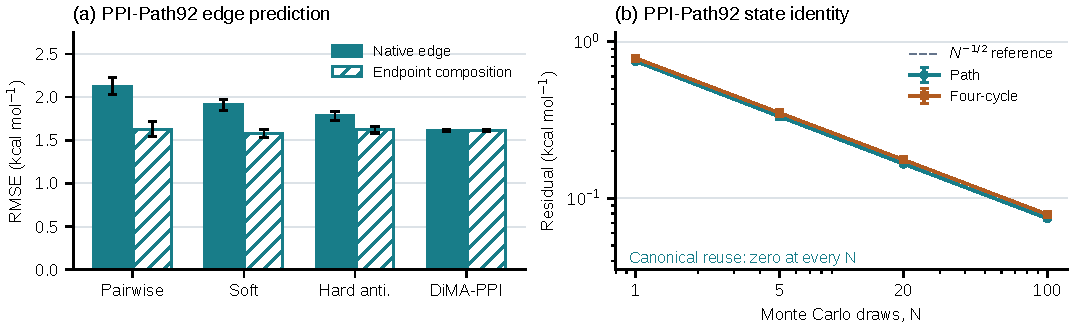
\includegraphics[width=\textwidth]{fig_results.pdf}
 \caption{Evaluation on PPI-Path92. (a) RMSE of native mutant-to-mutant
 predictions and composition of predicted WT effects, evaluated against
 differences of measured WT effects. Bars and error bars denote the mean
 and sample SD across five seeds. (b) Consistency residuals under independent
 state sampling with fixed StaB-ddG parameters. Canonical reuse yields zero
 measured residuals at all sample counts, as indicated below the curves.}
 \label{fig:results}
\end{figure*}
\subsection{Datasets and Evaluation Protocol}
\textbf{S1129.} The public benchmark contains 1,129 single substitutions
from 111 complexes following the two official exclusions from S1131. We use the five predefined complex-disjoint
outer folds from the DSSA-PPI protocol~\cite{dssappi}, with test sizes 169,
142, 271, 252 and 295. Approximately one eighth of each outer training fold
is reserved for validation using a seeded mutation-level split; complexes
may therefore occur in both fitting and validation subsets. We report the mean and sample SD across seeds 42--46 after averaging
per-fold metrics within each seed. PCC, Spearman correlation and RMSE
measure linear association, rank agreement and error magnitude, respectively.

\textbf{PPI-Path92.} We construct the Protein--Protein Interaction Mutation
Path Benchmark (PPI-Path92) from repeated-site measurements in S1129.
Measurements are grouped by complex, chain, PDB site and WT residue. Sites
with at least two distinct measured mutant variants are retained, with
duplicate records resolved by selecting the earliest source row. The resulting benchmark
contains 92 site panels from 27 complexes and 793 amino-acid states.
For each ordered mutant pair, the target is
\begin{equation}
 y^{\rm derived}_{b\to c}=y_{\mathrm{WT}\to c}-y_{\mathrm{WT}\to b}.
 \label{eq:path92target}
\end{equation}
PPI-Path92 contains 9,904 mutant-to-mutant comparisons with targets defined
by Eq.~\eqref{eq:path92target}. Native predictions evaluate each mutant pair
directly; endpoint composition subtracts the corresponding predicted WT
effects. Including WT edges, the state graphs contain
11,306 directed edges, supporting 5,653 reverse comparisons, 9,904 ordered
paths, 31,922 triangles and 133,736 four-state cycles per seed. Each panel
inherits the S1129 outer fold of its source complex, preserving
complex-disjoint evaluation.

Matched controls share residue-graph inputs and training settings: an
unconstrained pairwise regressor, reverse-label supervision, a soft reverse
consistency penalty (weight 0.20), hard pairwise antisymmetry, and a shared
potential without atomic state descriptors. Reverse and path residuals are
$|\widehat y_{a\to b}+\widehat y_{b\to a}|$ and
$|\widehat y_{a\to c}-\widehat y_{a\to b}-\widehat y_{b\to c}|$.
Cycle residuals are absolute sums around the loop.

\subsection{Comparison with Published Models and Ablation}
\begin{table}[t]
\centering
\caption{S1129 predictive accuracy: mean $\pm$ sample SD across five repeats or seeds, each averaged over five folds. RMSE is in kcal mol$^{-1}$.}
\label{tab:accuracy}
\footnotesize
\setlength{\tabcolsep}{3pt}
\begin{tabular}{lccc}
\toprule Model & PCC $\uparrow$ & Spearman $\uparrow$ & RMSE $\downarrow$ \\
\midrule
\multicolumn{4}{l}{\textit{Published-model comparison}} \\
DSSA-PPI~\cite{dssappi} & $0.706\pm0.011$ & $0.508\pm0.017$ & $1.717\pm0.040$ \\
DiMA-PPI (ours) & $0.757\pm0.009$ & $0.592\pm0.011$ & $1.542\pm0.023$ \\
\midrule
\multicolumn{4}{l}{\textit{Matched controls and ablation}} \\
Pairwise & $0.570\pm0.020$ & $0.514\pm0.021$ & $2.112\pm0.047$ \\
Reverse supervision & $0.756\pm0.009$ & $0.602\pm0.011$ & $1.565\pm0.039$ \\
Soft consistency & $0.759\pm0.012$ & $0.608\pm0.014$ & $1.551\pm0.045$ \\
Hard antisymmetry & $0.755\pm0.003$ & $0.594\pm0.009$ & $1.549\pm0.013$ \\
No state descriptors & $0.750\pm0.004$ & $0.578\pm0.006$ & $1.588\pm0.025$ \\
\bottomrule
\end{tabular}
\end{table}

DSSA-PPI~\cite{dssappi} is evaluated using five released repeats of
fold-specific checkpoints, using the same S1129 observations and outer
folds as DiMA-PPI and retaining its original pretraining and optimization
procedures.

DiMA-PPI achieves PCC $0.757\pm0.009$, Spearman correlation
$0.592\pm0.011$ and RMSE $1.542\pm0.023$~kcal mol$^{-1}$
(Table~\ref{tab:accuracy}). Relative to DSSA-PPI, DiMA-PPI increases
mean PCC by 0.051 and Spearman correlation by 0.084, and reduces RMSE by
0.176~kcal mol$^{-1}$. Among matched controls, soft consistency achieves the highest mean
PCC and Spearman correlation; DiMA-PPI achieves the lowest mean RMSE.

Removing state descriptors yields PCC 0.750, Spearman correlation 0.578
and RMSE 1.588. Paired uncertainty is estimated from five-seed ensemble
predictions using 10,000 complex-bootstrap replicates within each fold.
Including the descriptors increases ensemble PCC by 0.0098 (95\% CI 0.0002--0.0206) and reduces
RMSE by 0.0490~kcal mol$^{-1}$ (95\% CI 0.0138--0.0779).

\subsection{Path and Cycle Consistency on PPI-Path92}
\begin{table}[t]
\centering
\caption{PPI-Path92 mean absolute consistency residuals (kcal mol$^{-1}$), averaged across five seeds.}
\label{tab:consistency}
\footnotesize
\setlength{\tabcolsep}{3pt}
\begin{tabular}{lcccc}
\toprule Model & Reverse & Path & Triangle & Four-cycle \\
\midrule
Pairwise & $2.260$ & $1.298$ & $3.283$ & $4.248$ \\
Soft & $0.867$ & $0.879$ & $1.314$ & $1.652$ \\
Hard anti. & $1.63\!\times\!10^{-7}$ & $0.441$ & $0.305$ & $0.348$ \\
DiMA-PPI & $2.20\!\times\!10^{-7}$ & $4.78\!\times\!10^{-7}$ & $3.08\!\times\!10^{-7}$ & $3.68\!\times\!10^{-7}$ \\
\bottomrule
\end{tabular}
\end{table}

Table~\ref{tab:consistency} reports residuals for reversal, path composition
and cycle closure. Hard antisymmetry achieves numerical precision for
reversal, with mean path and four-cycle residuals of 0.441 and
0.348~kcal mol$^{-1}$. DiMA-PPI achieves mean residuals below
$5\times10^{-7}$ for all four relations. This evaluation recomputes scores
from deterministic canonical inputs for each requested edge; the resulting
residuals are consistent with floating-point arithmetic.

\subsection{Compositional Prediction on PPI-Path92}
On the 9,904 mutant-to-mutant edges defined by
Eq.~\eqref{eq:path92target}, native pairwise, soft, hard and DiMA-PPI
predictors achieve PCC 0.354, 0.442, 0.502 and 0.547, and RMSE 2.128, 1.910,
1.783 and 1.611~kcal mol$^{-1}$, respectively (Fig.~\ref{fig:results}a).
The paired bootstrap of five-seed ensemble predictions estimates an RMSE
reduction of 0.167 (95\% CI 0.016--0.466) relative to hard antisymmetry. The ensemble
PCC gain is 0.049 (95\% CI $-0.041$ to 0.175).

Composition of predicted WT effects yields RMSE 1.630, 1.578 and 1.622
for the pairwise, soft and hard controls, respectively. Endpoint composition
therefore recovers much of the accuracy difference observed for native
predictions; the composed soft control has the lowest mean RMSE. In
DiMA-PPI, native prediction and endpoint composition are algebraically
equivalent through the shared state potential.

\subsection{Effect of Canonical State Reuse}
We assess the effect of state reuse with 25 fixed StaB-ddG checkpoints
covering five folds and five seeds. Independent and canonical inference use
the same panels and nested Monte Carlo sample counts
$N\in\{1,5,20,100\}$. Independent mean path error decreases from 0.751 to
0.074~kcal mol$^{-1}$, approximately following $N^{-1/2}$
(Fig.~\ref{fig:results}b). Reusing each state estimate across edges
yields zero measured reverse, path and cycle residuals at every $N$.
In the paired evaluation at $N=20$, canonical reuse preserves the
WT-to-mutant estimates and their predictive metrics while enforcing
closure across the state graph.

A computational evaluation using the seed-42 DiMA-PPI checkpoints covers
793 amino-acid states, 1,586 bound/free contexts and 11,306 directed edges
in PPI-Path92. Independent edge evaluation
requests 45,224 context scores; canonical reuse requires 1,586, a
28.5-fold reduction. On an Intel Core i7-12700KF with eight PyTorch CPU
threads and batch size 32, model inference time decreases from 469.4 to
16.1 seconds, corresponding to a 29.1-fold speedup. Checkpoint/cache loading, graph assembly and disk
I/O are performed outside the timed region. The mean and maximum absolute
prediction differences between the two inference procedures are $1.10\times10^{-7}$
and $1.67\times10^{-6}$~kcal mol$^{-1}$, and reused scores give zero measured
closure residuals.

\section{Discussion and Conclusion}
DiMA-PPI combines a shared four-state encoder with canonical state identity
to produce globally consistent mutation predictions. It achieves PCC 0.757
on S1129 and RMSE 1.611 on the PPI-Path92 compositional benchmark, with
path and cycle residuals at numerical precision. Fixed-weight experiments
establish canonical scalar reuse as an effective way to preserve consistency
and reduce repeated inference across state graphs.

Extensions to condition-aware states, conformational ensembles and
multi-site mutation paths provide further directions for evaluation.

\section*{Acknowledgment}
OpenAI Codex assisted with manuscript drafting, formatting and result-summary
visualization.
\bibliographystyle{IEEEtran}
\bibliography{dima_full_references}
\end{document}
